%Template file for a presentation using Latex and beamer
%You will need to install Latex, the beamer package, and some of these other packages on your own.
\documentclass[11pt,compress]{beamer} %slides and notes
\usepackage{amsmath,datetime,array,alltt,graphicx,xmpmulti,mathtools,bbm,booktabs,xspace,mathabx,tikz,pifont,epstopdf,relsize,wedn,hyperref,framed}
\usepackage[justification=centering]{caption}
\usepackage{subcaption}\captionsetup{compatibility=false}
\usepackage[autolinebreaks]{mcodefred}
\usepackage[author-year]{amsrefs}
\usepackage{qtree}
\usepackage{pst-node}% http://ctan.org/pkg/pst-node
\usepackage{textcomp} %helps to compile MATLAB code in mcode or lstlisting
\usepackage{pgf,pgfarrows,pgfnodes} % Drawing tables, arrows, ...
\usepackage[customcolors]{hf-tikz} % Box equations
\input FJHDef.tex


\newcommand{\HickernellFJ}{Hickernell} %To give my name to the bibliography

\newtheorem{lem}{Lemma}
\setbeamertemplate{theorems}[numbered]

\usetikzlibrary{arrows}
\newcommand*\circled[1]{\tikz[baseline=(char.base)]{
  \node[shape=circle,color=green,draw,inner sep=1pt] (char) {#1};}}
\setlength{\parskip}{2ex}
\setlength{\arraycolsep}{0.5ex}
\newcommand{\tol}{\text{tol}}
\newcommand{\e}{\text{e}}
\DeclareMathOperator{\cubMC}{cubMC}
\DeclareMathOperator{\qse}{qse}
\DeclareMathOperator{\integ}{int}
\DeclareMathOperator{\trap}{trap}
\DeclareMathOperator{\size}{size}
\DeclareMathOperator{\app}{id}
\DeclareMathOperator{\err}{err}
\DeclareMathOperator{\walsh}{walsh}
\newcommand{\happ}{\widehat{\app}}
\newcommand{\hinteg}{\widehat{\integ}}
\newcommand{\cube}{[0,1)^d}
\newcommand{\desall}{\{\vx_i\}}
\newcommand{\desn}{\{\vz_i\}_{i=0}^{n-1}}
\def\newblock{\hskip .11em plus .33em minus .07em}
\newcommand{\wcS}{\widecheck{S}}
\newcommand{\wcomega}{\widecheck{\omega}}
\newcommand{\prob}[1]{\mathbb{P}\left( #1 \right)}
\newcommand{\bsk}{\boldsymbol{k}}    % vector k
\newcommand{\bsz}{\boldsymbol{z}}    % vector z
\newcommand{\bsx}{\boldsymbol{x}}    % vector z
\newcommand{\F}{\mathbb{F}} % field, finite field
\newcommand{\bsDelta}{\boldsymbol{\Delta}}    % vector
\newcommand{\bszero}{\boldsymbol{0}} % vector of zeros
\newcommand{\E}{{\rm e}}
\newcommand{\D}{{\rm d}}
\newcommand{\Z}{\mathbb{Z}}
\newcommand{\R}{\mathbb{R}}
\newcommand{\N}{\mathbb{N}}
\newcommand{\I}{\mathsf{I}}
\DeclareMathOperator{\Var}{Var}
\DeclareMathOperator{\affine}{affine}
\DeclareMathOperator{\Genz}{Genz}
\DeclareMathOperator{\payoff}{payoff}
\newcommand{\intalg}{\hI\left(\vx\mapsto f(\vx),\varepsilon_a\right)}

\definecolor{orange_plot}{rgb}{1.,.5,.0}
\definecolor{gray_plot}{rgb}{.7,.7,.7}
\definecolor{green_plot}{rgb}{.0,.5,.0}


\usetheme{FredIIT}
% \usetheme{Berlin}
\logo{\includegraphics[width=1cm]{MengerIITRedGray.pdf}}

\title[JSM 2016]{Automatic estimation of Sobol' indices based on quasi-Monte Carlo methods}
\author[ljimene1@hawk.iit.edu]{Llu\'is Antoni Jim\'enez Rugama\\Joint work with: Elise Arnaud (Univ. Grenoble),\\Laurent Gilquin (Univ. Grenoble), Fred J. Hickernell (IIT), \\Herv\'{e} Monod (INRA), and Cl\'ementine Prieur (Univ. Grenoble)}
\institute{Room 120, Bldg E1, Department of Applied Mathematics \\
Illinois Institute of Technology, Chicago, 60616 IL \\
Email: \href{mailto:ljimene1@hawk.iit.edu}{\url{ljimene1@hawk.iit.edu}}}
%Website: \url{http://math.iit.edu/~lantoni/}
% \date[{Revised \currenttime, \mdyyyydate \today}]{Revised \settimeformat{ampmtime} \currenttime, \today}
%\date[]{\today}
\date[]{Tuesday ${\rm{2^{nd}}}$ August, 2016}

\begin{document}
\frame{\titlepage}

%\frame{\frametitle{Outline}\begin{minipage}{15cm}\tableofcontents\end{minipage}}
%\AtBeginSection[]
%{ \begin{frame}
%  \frametitle{Outline}
%  \begin{minipage}{15cm}
%  \tableofcontents[currentsection]
%  \end{minipage}
%  \end{frame}
%}

\begin{frame}<1>[label = Outline]\frametitle{Outline}
\begin{itemize}
\item<1,2> \alert<2>{Introduction}\only<2>{---The ANalysis Of VAriance.}
\item<1,3> \alert<3>{Sobol' Indices}\only<3>{---Measuring the importance of each input.}
\item<1,4> \alert<4>{Quasi-Monte Carlo Methods}\only<4>{---How can we estimate integrals in high dimensions?}
\item<1,5> \alert<5>{Numerical example}\only<5>{---The \ocite{BraFoxNie92} function}
\end{itemize}
\end{frame}

\section{Introduction}
\setbeamercovered{transparent} % Translucid <only>
\againframe<2>{Outline}
\setbeamercovered{invisible} % Invisible <only>

\begin{frame}
\frametitle{ANOVA}
For $f\in L^2\left([0,1]^d\right)$, and $1:d=\{1,\dots,d\}$,
\begin{equation*}
f(\vx)=\sum \limits_{u \subseteq 1:d} f_u(\vx)\, , \qquad f_{\varnothing} = \mu\, ,
\label{anova}
\end{equation*}
where,
\[f_u(\vx)= \int_{[0,1]^{d-|u|}} f(\vx) d{\vx}_{-u} - \sum \limits_{v \subset u} f_v(\vx)\, .\]

\begin{itemize}
\item $\abs{u}$ the cardinality of $u$.
\item $-u:=u^c$.
\end{itemize}
\end{frame}

\begin{frame}
\frametitle{Variance Decomposition}
Under the previous definitions,
\begin{equation*}
\sigma^2_{\varnothing} = 0\, ,\qquad \sigma^2_{u} =\int_{[0,1]^{d}} f_u(\vx)^2 d{\vx}\, ,\qquad \sigma^2 =\int_{[0,1]^{d}} \left(f(\vx)-\mu\right)^2 d{\vx}\, .
\end{equation*}
The ANOVA identity is,

\[
\sigma^2 = \sum \limits_{u \subseteq1:d} \sigma_u^2 \, .
\]
\end{frame}

\section{Sobol Indices'}
\setbeamercovered{transparent} % Translucid <only>
\againframe<3>{Outline}
\setbeamercovered{invisible} % Invisible <only>

\begin{frame}
\frametitle{Sobol' Indices for Uncertainty Quantification}
We consider the random variable $Y=f(\vX)$ with $\vX\sim U\left([0,1)^d\right)$.

Sobol' introduced the \emph{global sensitivity} indices which measure the variance explained by any dimension subset $u\subseteq 1:d$:
\begin{equation*}
\underline{\tau}_u^2 = \sum_{\substack{v \subseteq u \\ v\,\subseteq 1:d}} \sigma_v^2\, , \quad \text{ and } \quad \overline{\tau}_u^2 = \sum_{\substack{v \cap u\neq\varnothing \\ v\,\subseteq 1:d}} \sigma_v^2\, .
\end{equation*}
We have the following properties,
\begin{itemize}
\item $\underline{\tau}_u^2\leq \overline{\tau}_u^2$.
\item $\underline{\tau}_u^2 + \overline{\tau}_{-u}^2 =\sigma^2$.
\end{itemize}
\end{frame}

\begin{frame}
\frametitle{Estimation of the Integral}
Indices $\underline{\tau}_u^2$ and $\overline{\tau}_u^2$ can be estimated with integrals:
\begin{align*}
\underline{\tau}_u^2  &= \int_{[0,1]^{2d-1}} f(\vx)f(\vx_{u}:{\vx'}_{-u})d\vx d{\vx'} - \left(\int_{[0,1]^d}f(\vx) d\vx\right)^2, \\
\overline{\tau}_u^2 &= \frac{1}{2}\int_{[0,1]^{d+1}}\left(f(\vx')-f(\vx_u:{\vx'}_{-u})\right)^2 d\vx d{\vx'}.
\end{align*}
where the point $\vz := (\vx_u:{\vx'}_{-u})$ has coordinates $z_j=x_j$ if $j\in u$, and $z_j={x'}_j$ if $j\notin u$.

\end{frame}

%\begin{frame}
%\frametitle{Sobol' Indices}
%For $\vX\sim U[0,1]^d$, we are interested in estimating the \emph{first-order} and \emph{total-effect} normalized indices,
%\setbeamercovered{transparent} % Translucid <only>
%\begin{gather*}
%\underline{\tau}_u^{2,*}=\frac{\Var \left[ \mathbb{E} \left(f({\vX})|{\vX}_{u}\right)\right] }{\Var\left(f({\vX})\right)}\uncover<1>{=
%1-\frac{\mathbb{E}\left[ \Var \left(f({\vX})|\vX_u\right)\right]}{\Var\left(f({\vX})\right)},}\\
%\uncover<1>{\overline{\tau}_u^{2,*}=1-\frac{\Var \left[ \mathbb{E} \left(f({\vX})|\vX_{-u}\right)\right]}{\Var\left(f({\vX})\right)}=\frac{\mathbb{E}\left[ \Var \left(f({\vX})|{\vX}_{-u}\right)\right] }{\Var\left(f({\vX})\right)}.}
%\end{gather*}
%satisfying $
%0\leq \underline{\tau}_u^{2,*} \leq \overline{\tau}_u^{2,*}\leq 1$.\setbeamercovered{invisible} % Invisible <only>
%\vspace{-0.2cm}
%\uncover<2>{The \emph{first-order} indice is composed by,
%\begin{equation*}
%\underline{\tau}_u^{2,*}=\frac{I^{(1)}}{I^{(2)}-\left(I^{(3)}\right)^2},\quad \text{where }\begin{cases}I^{(1)}\text{ is a }2d-1\text{ dim. integral.} \\ I^{(2)}\text{ is a }d\text{ dim. integral.} \\ I^{(3)}\text{ is a }d\text{ dim. integral.} \end{cases}
%\end{equation*}
%%\vspace{-0.3cm}
%Error bounds for $\underline{\tau}_u^2$ require more care than error bounds for $I^{(k)}$.
%}
%\end{frame}

\section{Quasi-Monte Carlo Methods}
\setbeamercovered{transparent} % Translucid <only>
\againframe<4>{Outline}
\setbeamercovered{invisible} % Invisible <only>

\begin{frame}
\frametitle{Numerical Integration Problem}
Given $\varepsilon_a$ and $\vx\mapsto f(\vx)$, we want $\hI$ such that
\[
\abs{\int_{\cube} f(\bsx)\,\D\bsx - \intalg}\leq \varepsilon_a,
\]
where
\[
\intalg = \frac{1}{2^m} \sum_{i=0}^{2^m-1} f(\bsz_i \oplus\bsDelta),
\]
for some \alert{automatic} and \alert{adaptive} choice of $m$, $\{\bsz_i\}_{i=0}^{\infty}
\in\begin{Bmatrix}\textcolor{magenta}{\text{Lattice}}\\\textcolor{blue}{\text{Digital}}\end{Bmatrix}$ sequence, and
\[
\cost\left(\intalg\right)=\mathcal{O}\left((m+\$(f))2^m\right)
\]
\end{frame}

\begin{frame}
\frametitle{Examples of Sequences}
\begin{figure}\centering
\begin{subfigure}[b]{0.45\textwidth}
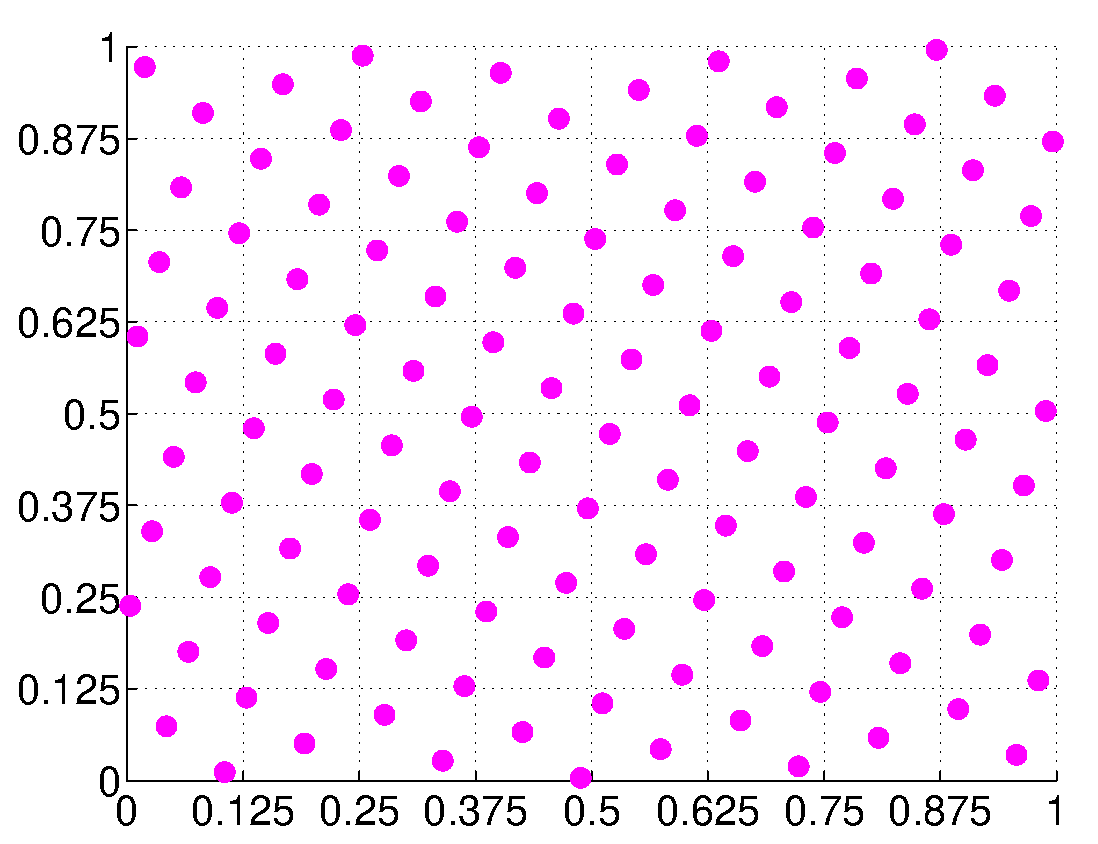
\includegraphics[width=1.\textwidth]{Images/lat_seq.eps}
\caption*{Shifted rank-1 lattice sequence with generating vector $(1,47)$.}
\end{subfigure}
~ % Spacing between figures
\begin{subfigure}[b]{0.45\textwidth}
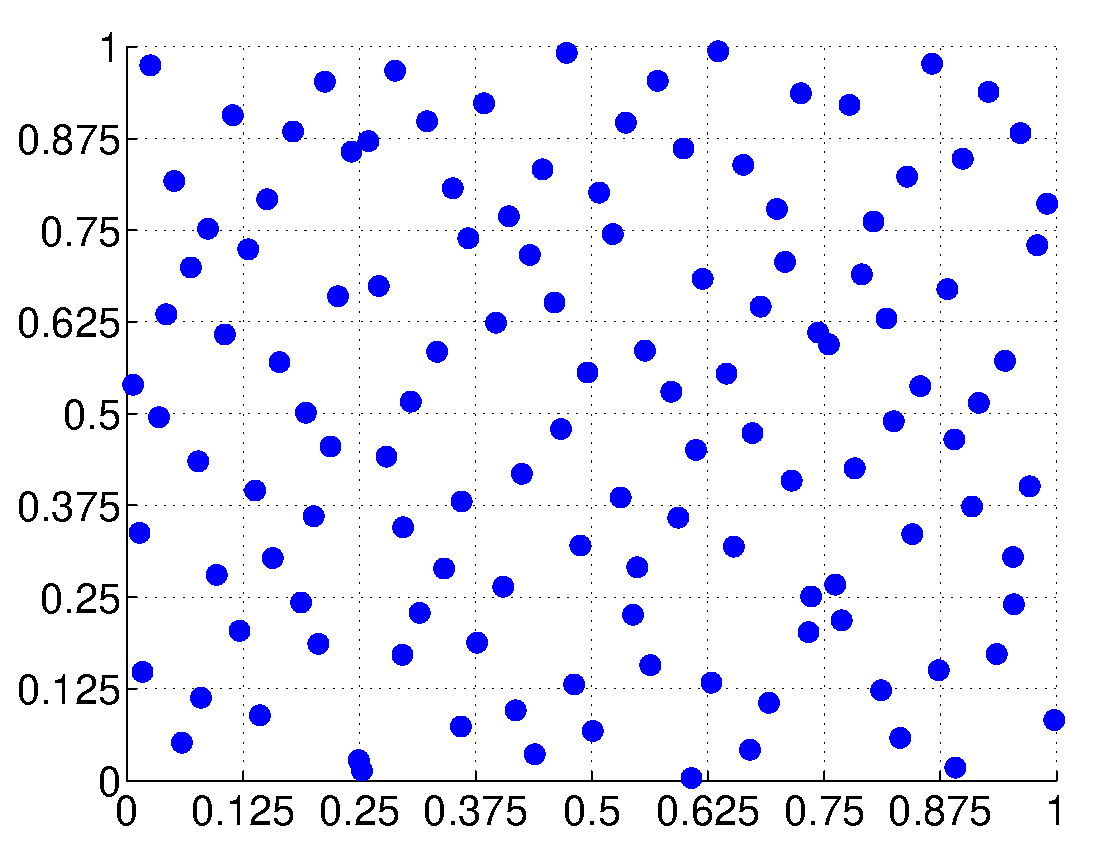
\includegraphics[width=1.\textwidth]{Images/sob_seq.eps}
\caption*{Digitally shifted scrambled Sobol' sequence.}
\end{subfigure}
\end{figure}
\end{frame}

\begin{frame}
\frametitle{Adaptive Algorithm}
The idea behind the results in \ocite{JimHic16a} and \ocite{HicJim16a} is that for all $f\in\cc$,
\[
\abs{\int_{\cube} f(\bsx)\,\D\bsx - \intalg}\leq a(r,m)\sum_{\kappa=\left \lfloor 2^{m-r-1}\right \rfloor}^{2^{m-r}-1} \bigabs{\tf_{m,\kappa}}.
\]
\begin{itemize}
\item $\tf_{m,\kappa}=$ discrete Fourier $\begin{Bmatrix}\textcolor{magenta}{\text{Exponential}}\\\textcolor{blue}{\text{Walsh}}\end{Bmatrix}$ coefficients of $f$.
\item $a(r,m)=$ inflation factor that depends on $\cc$.
\end{itemize}
\end{frame}

%\begin{frame}
%\frametitle{IID Monte Carlo Error Depends on All Fourier Coefficients}
%In the Monte Carlo case, if $I(f)=\int_{\cube} f(\vx)\,\D\vx$,
%\[
%\mathbb{E}\left[\left(I(f) - \frac{1}{2^m} \sum_{i=0}^{2^m-1} f(\vz_i)\right)^2 \right]\leq \frac{1}{2^m}\overbrace{\sum_{\kappa\neq 0} \abs{\hf_{\kappa}}^2}^{\Var\left[f(\vZ)\right]}
%\]
%\begin{itemize}
%\item $\vz_i$ are IID samples with distribution $U[0,1]^d$.
%\item $f(\vz)=\sum_{\kappa}\hf_{\kappa}\phi(\vz)$ is the Fourier decomposition of $f(\vz)$.
%\end{itemize}
%\end{frame}

\begin{frame}
\frametitle{QMC Error Bounds Depend Only on Some Fourier Coefficients for $f\in\cc$}
In the quasi-Monte Carlo case,
\[
\abs{I(f) - \frac{1}{2^m} \sum_{i=0}^{2^m-1} f(\bsz_i \oplus\bsDelta)}\leq \sum \textcolor{green_plot}{\boldsymbol{\bigcirc}}\leq
a(r,m)\sum_{\kappa=\left \lfloor 2^{m-r-1}\right \rfloor}^{2^{m-r}-1} \bigabs{\tf_{m,\kappa}}
\]
\vspace{-.5cm}
\begin{columns}
\begin{column}{0.6\textwidth}
\centering
\begin{figure}
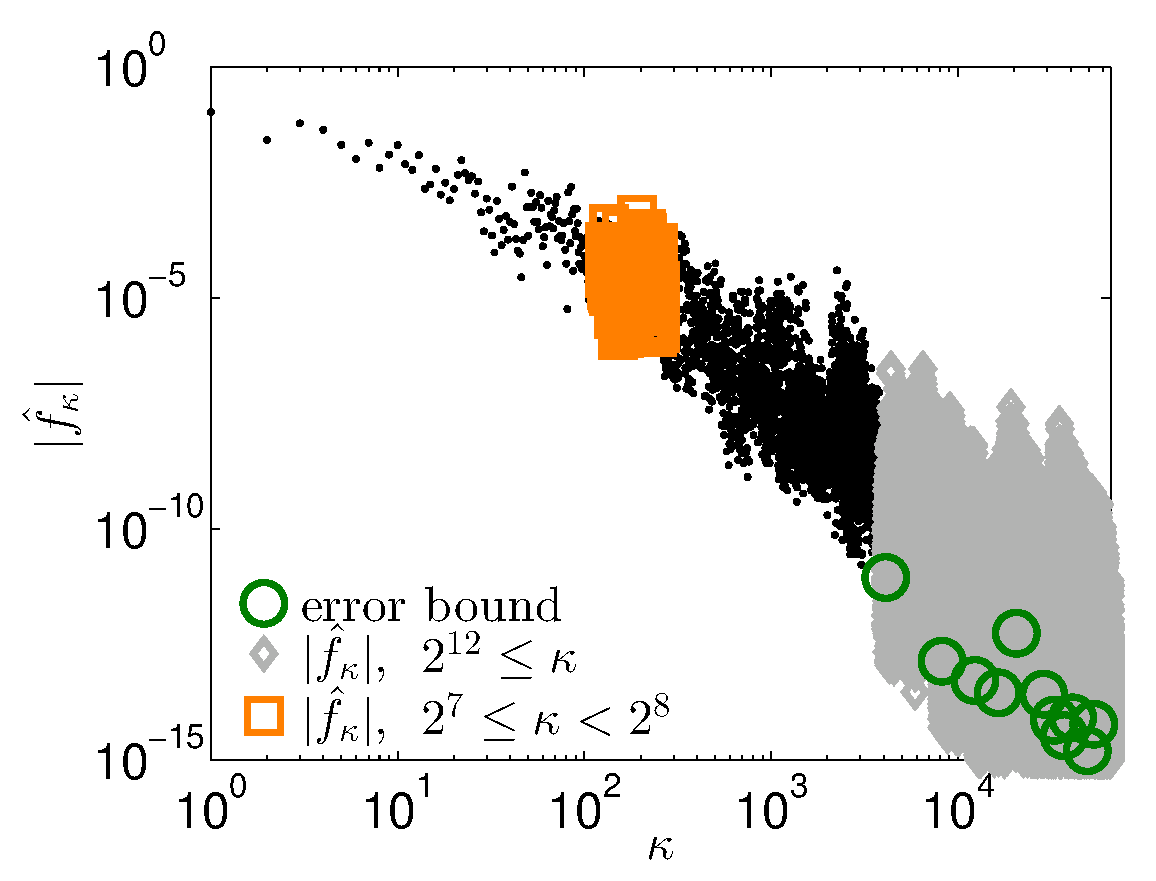
\includegraphics[width=.8\textwidth]{Images/WalshCoeffExplanation.eps}
\end{figure}
\end{column}
\begin{column}{0.4\textwidth}
\centering
$\cc=\begin{Bmatrix}\displaystyle\sum\textcolor{orange_plot}{\pmb{\Box}}\text{ bounds }\sum\textcolor{gray_plot}{\boldsymbol{\Diamond}}\\
\displaystyle\sum\textcolor{gray_plot}{\boldsymbol{\Diamond}}\text{ bounds }\sum\textcolor{green_plot}{\boldsymbol{\bigcirc}}\end{Bmatrix}$
\end{column}
\end{columns}
\end{frame}

\section{Numerical Example}
\setbeamercovered{transparent} % Translucid <only>
\againframe<5>{Outline}
\setbeamercovered{invisible} % Invisible <only>

\begin{frame}
\frametitle{\ocite{BraFoxNie92}}
\vspace{-0.5cm}
\[
f(\vX)=\sum_{i=1}^6 (-1)^i \prod_{j=1}^i \vX_j=-\vX_1+\vX_1\vX_2-\vX_1\vX_2\vX_3+\dots
\]
\begin{equation*}
\begin{array}{ c | c | c | c | c | c | c }
	\rm{Values} & j=1  &  j=2 &	j=3 &  j=4 &  j=5	& j=6 \\
  \hline			
    S_j & 65.3\%   & 17.9\%   & 3.7\%  &  1.3\%  &  0.1\%  &  0.1\% \\
    S_{j}^{\textup{tot}} & 74.0\%  &  26.6\%  &  7.7\%  &  3.3\%  &  0.6\%  &  0.7\% \\
  \hline  
\end{array}
\end{equation*}
\begin{equation*}
\begin{array}{ c | c | c | c | c | c | c }
	n & j=1  &  j=2 &	j=3 &  j=4 &  j=5	& j=6 \\
  \hline			
    S_j & 65536   & 32768   & 16384  &  8192  &  2048  &  1024 \\
    S_{j}^{\textup{tot}} & 32768  &  16384  &  8192  &  4096  &  1024  &  1024 \\
  \hline  
\end{array}
\end{equation*}

Computation time was 0.37 seconds for $\varepsilon_a=10^{-3}$.
\end{frame}

\begin{frame}
\frametitle{Conclusions and Future Work}
\begin{itemize}
\item The Sobol' indices algorithm accepts user input \alert{relative error} tolerances.
\item The estimation can be performed over the \alert{normalized} indices.
\item First-order indices can also be estimated using the \alert{replicated method} because quasi-Monte Carlo methods are \alert{compatible} with the replicated method.
\end{itemize}
\end{frame}


\part{References}
\begin{frame}[allowframebreaks]\frametitle{References}
\nocite{Owen2013VCG,Sobol01Global,HicJim16a,Nie92}
\bibliography{FJHown23,FJH22,lluisantoni}
\end{frame}

\begin{frame}
\frametitle{Inside and Outside $\cc$}
\begin{figure}\centering
\begin{subfigure}[b]{0.35\textwidth}
\includegraphics[width=1.\textwidth]{Images/fuzzy_FunctionWalshFourierCoeffDecay.eps}
\end{subfigure}
~ % Spacing between figures
\begin{subfigure}[b]{0.35\textwidth}
\includegraphics[width=1.\textwidth]{Images/fuzzy_FilteredFunctionWalshFourierCoeffDecay.eps}
\end{subfigure}
\end{figure}
\vspace{-.5cm}
\begin{figure}\centering
\begin{subfigure}[b]{0.35\textwidth}
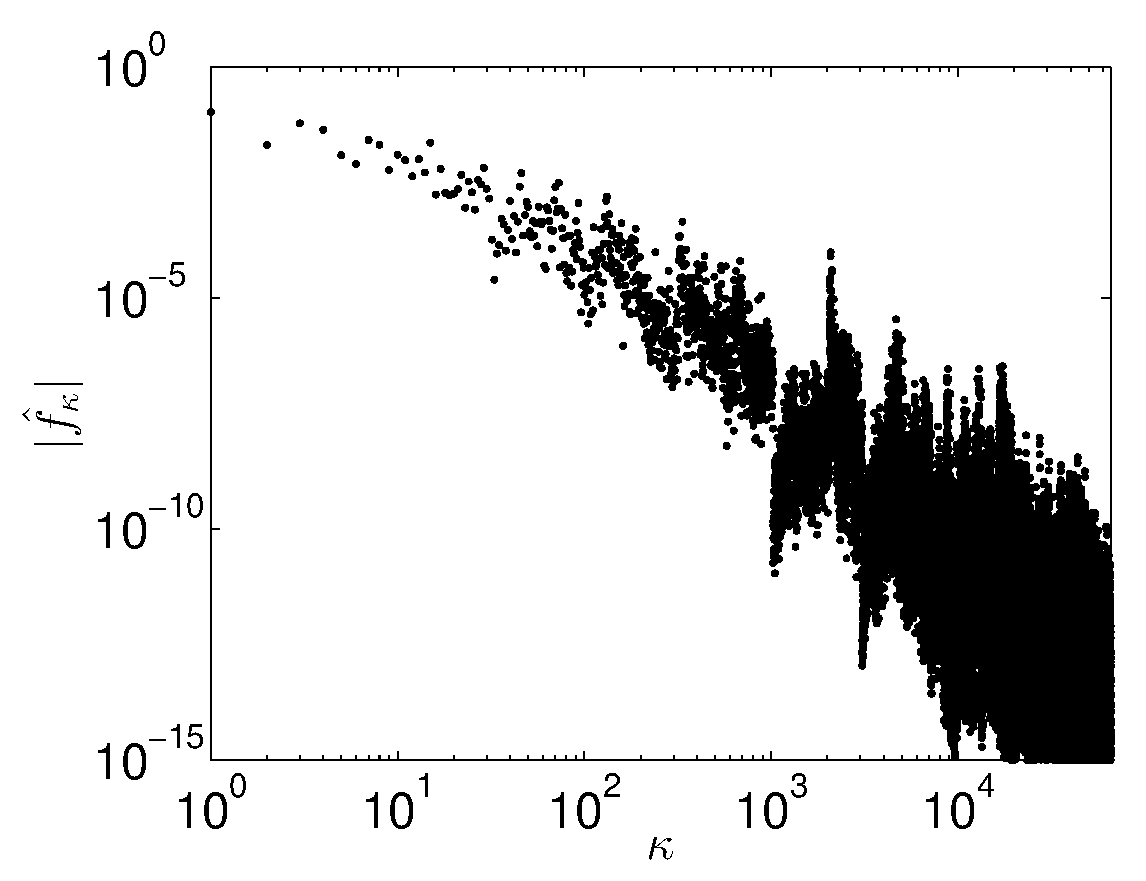
\includegraphics[width=1.\textwidth]{Images/WalshFourierCoeffDecayFilter.eps}
\end{subfigure}
~ % Spacing between figures
\begin{subfigure}[b]{0.35\textwidth}
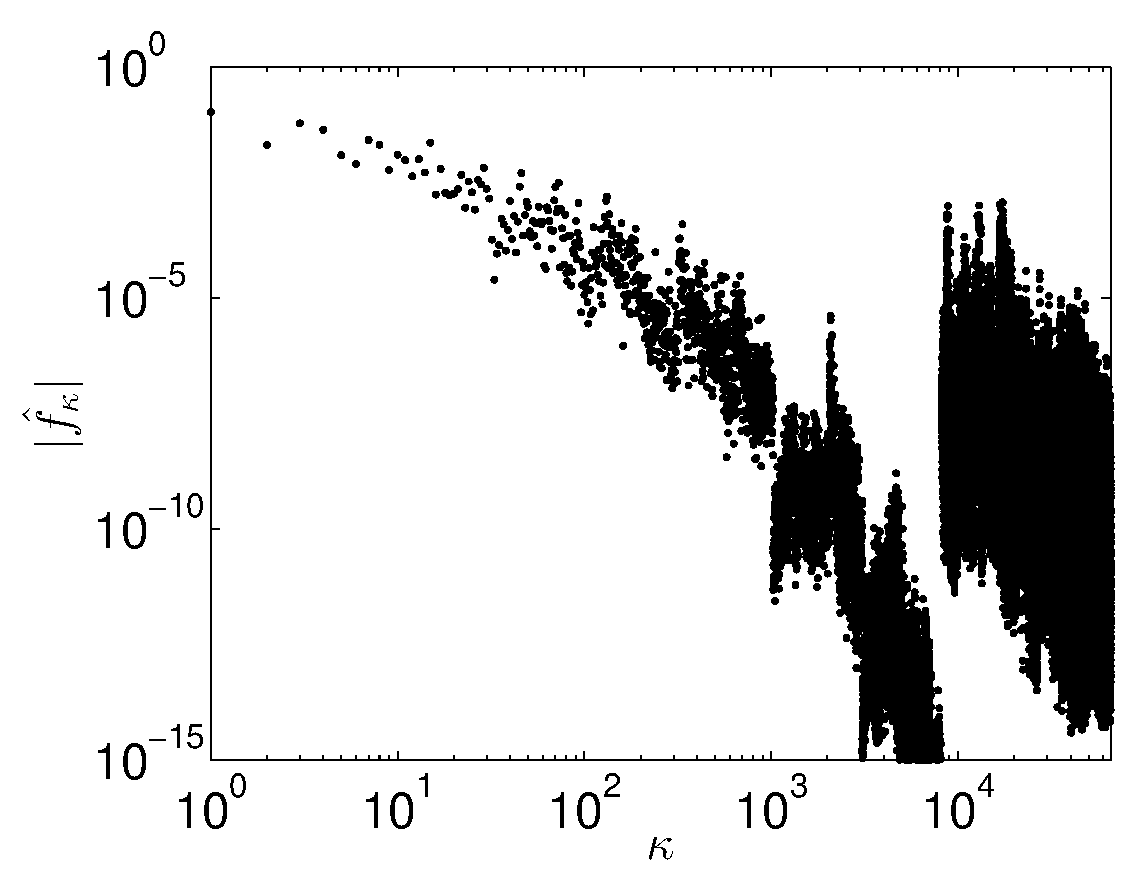
\includegraphics[width=1.\textwidth]{Images/fuzzy_WalshFourierCoeffDecayFilter.eps}
\end{subfigure}
\end{figure}
\end{frame}

\end{document}
